\documentclass[11pt,a4paper]{article}
\usepackage{polski}
\usepackage[utf8]{inputenc}
\usepackage{listings}
\usepackage{graphicx}
\usepackage{color}
\title{Dźwięk i muzyka w systemach komputerowych - laboratorium 01}
\author{Marcin Fabrykoski}
\begin{document}
\maketitle
\newpage
\begin{enumerate}
\item Naszym zadaniem jest wygenerowanie sygnału o częstotliwości 1kHz próbkowanego z częstotliwością 48kHz. Obliczenie transformaty Fouriera.\\
Kod realizujący to zadanie w MatLabie został przedstawiony poniżej:
\lstinputlisting[language=Octave,basicstyle=\footnotesize,caption="Zadanie 1"]{proba1.m}
czego wynik przestawia rys \ref{fig:a1}\\
\begin{figure}
\centering
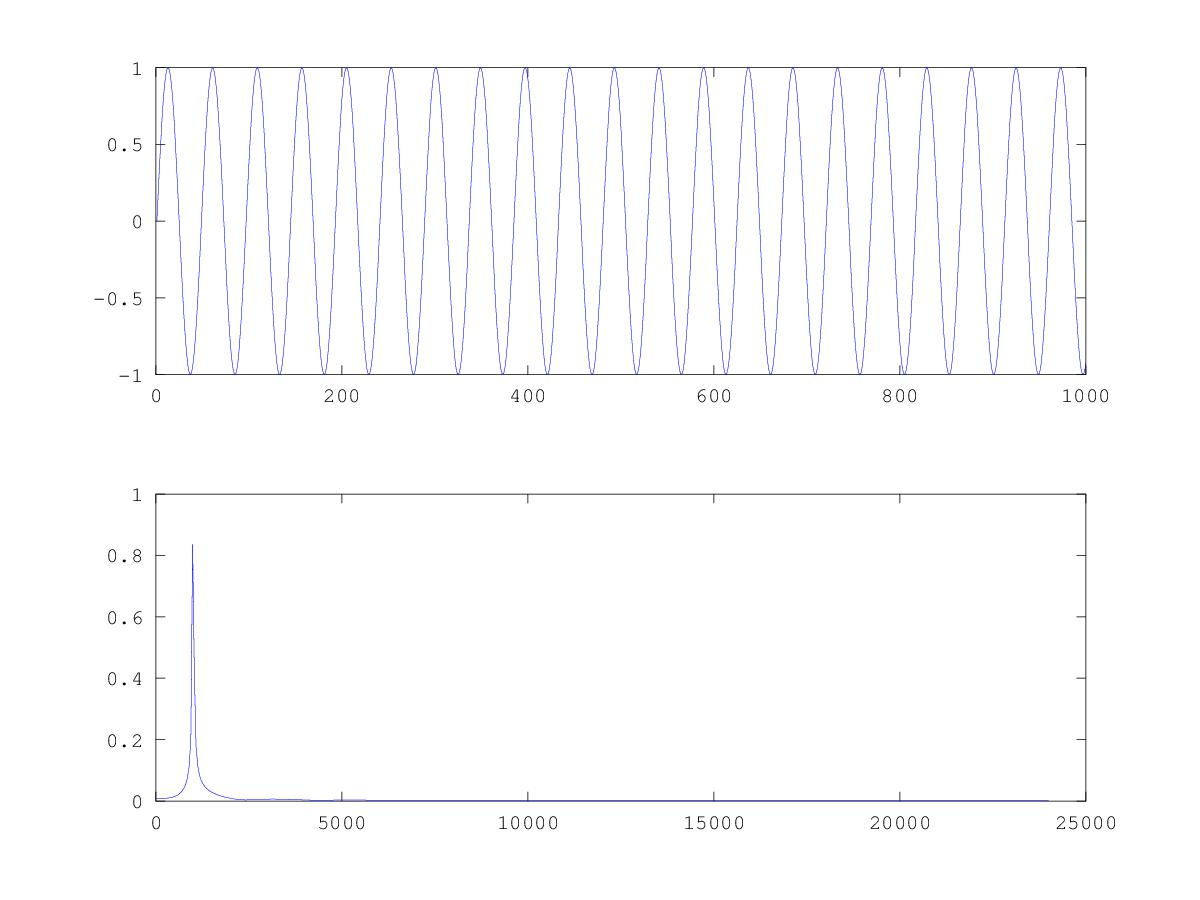
\includegraphics[scale=0.8]{proba1_dom}
\caption{Sygnał sinusoidalny i jego transformata Fouriera}
\label{fig:a1}
\end{figure}
Podczas zmniejszenia liczby próbek do 100, obserwujemy szumy w transformacie: rys. \ref{fig:a2}\\
\begin{figure}
\centering
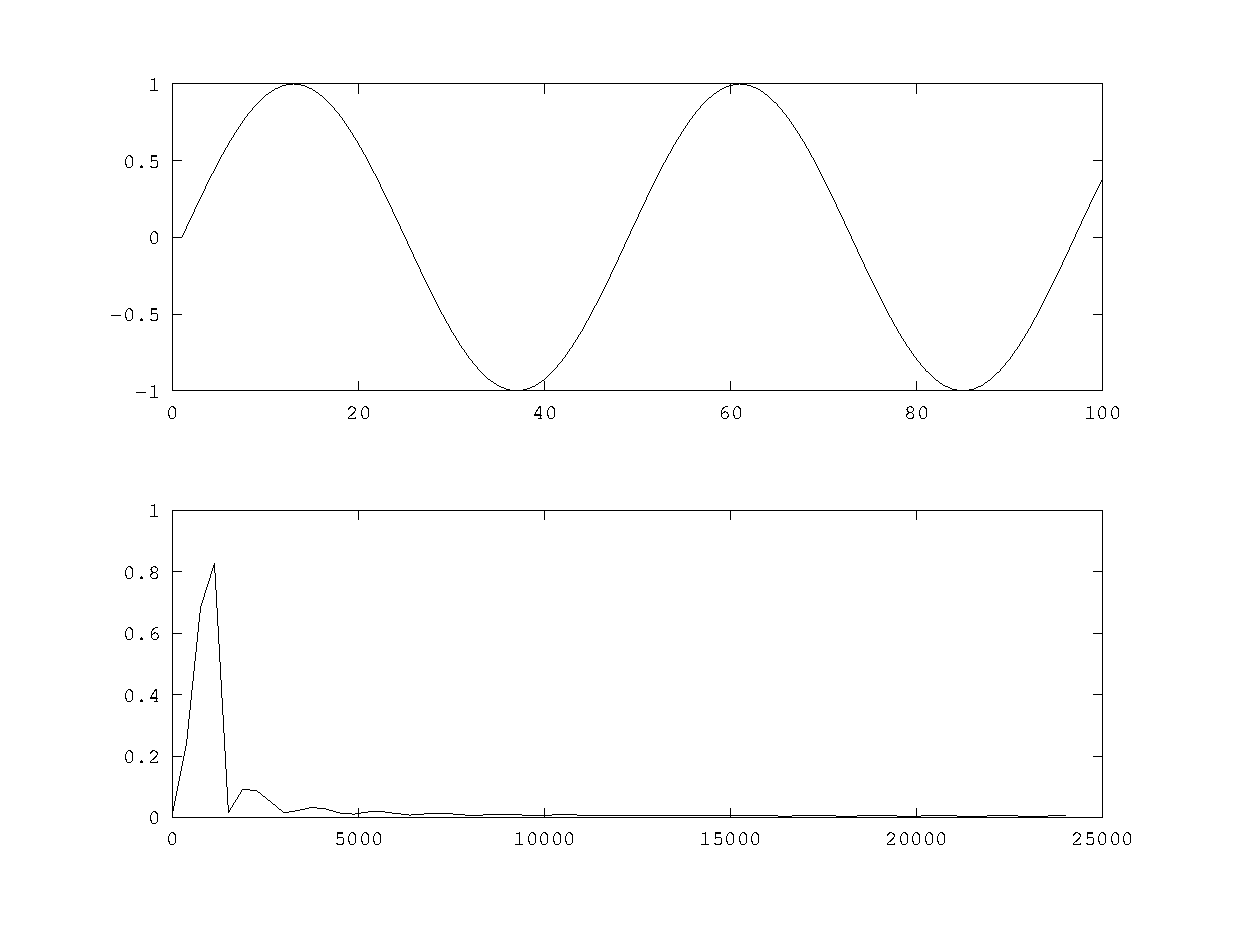
\includegraphics[scale=0.8]{proba1_2_dom}
\caption{Sygnał sinusoidalny i jego transformata - 100 próbek}
\label{fig:a2}
\end{figure}
Natomiast dla 100000 próbek otrzymujemy rys. \ref{fig:a3}
\begin{figure}
\centering
\includegraphics[scale=0.8]{proba1_3_dom}
\caption{Sygnał sinusoidalny i jego transformata - 100000 próbek}
\label{fig:a3}
\end{figure}
\newpage
\item Celem tego zadania jest zsumowanie dwóch sygnałów sinusoidalnych o takich samych amplitudach, lecz różnych częstotliwościach. Zadanie to realizuje poniższy program:
\lstinputlisting[language=octave,basicstyle=\footnotesize,caption="Zadanie 2"]{proba2.m}
Czego wynik możemy zaobserwować na rys. \ref{fig:4}
\begin{figure}
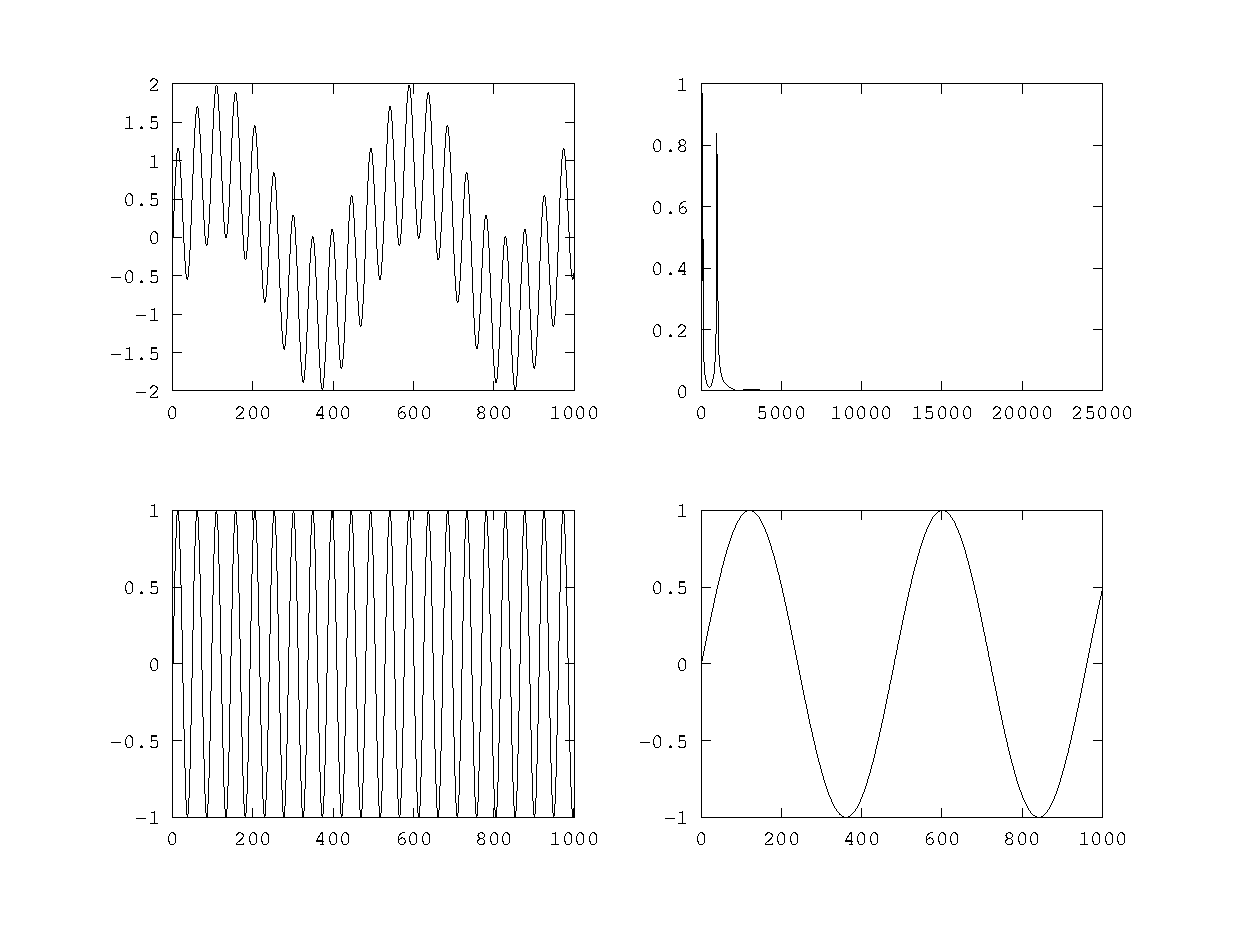
\includegraphics[scale=0.8]{proba2_dom}
\caption{Suma dwóch sygnałów sinusoidalnych}
\label{fig:4}
\end{figure}
\newpage
\item W tym ćwiczeniu należy zmodulować amplitudowo sygnał. W naszym zadaniu będziemy używać dwóch sygnałów o takich samych amplitudach, natomiast różnych częstotliwościach, odpowiednio: 100Hz i 1000Hz. Powyższe zadanie realizuje program:
\lstinputlisting[language=octave,basicstyle=\footnotesize,caption="Zadanie 3"]{proba3.m}
Czego wynik można przedstawić graficznie na rys. \ref{fig:5}
\begin{figure}
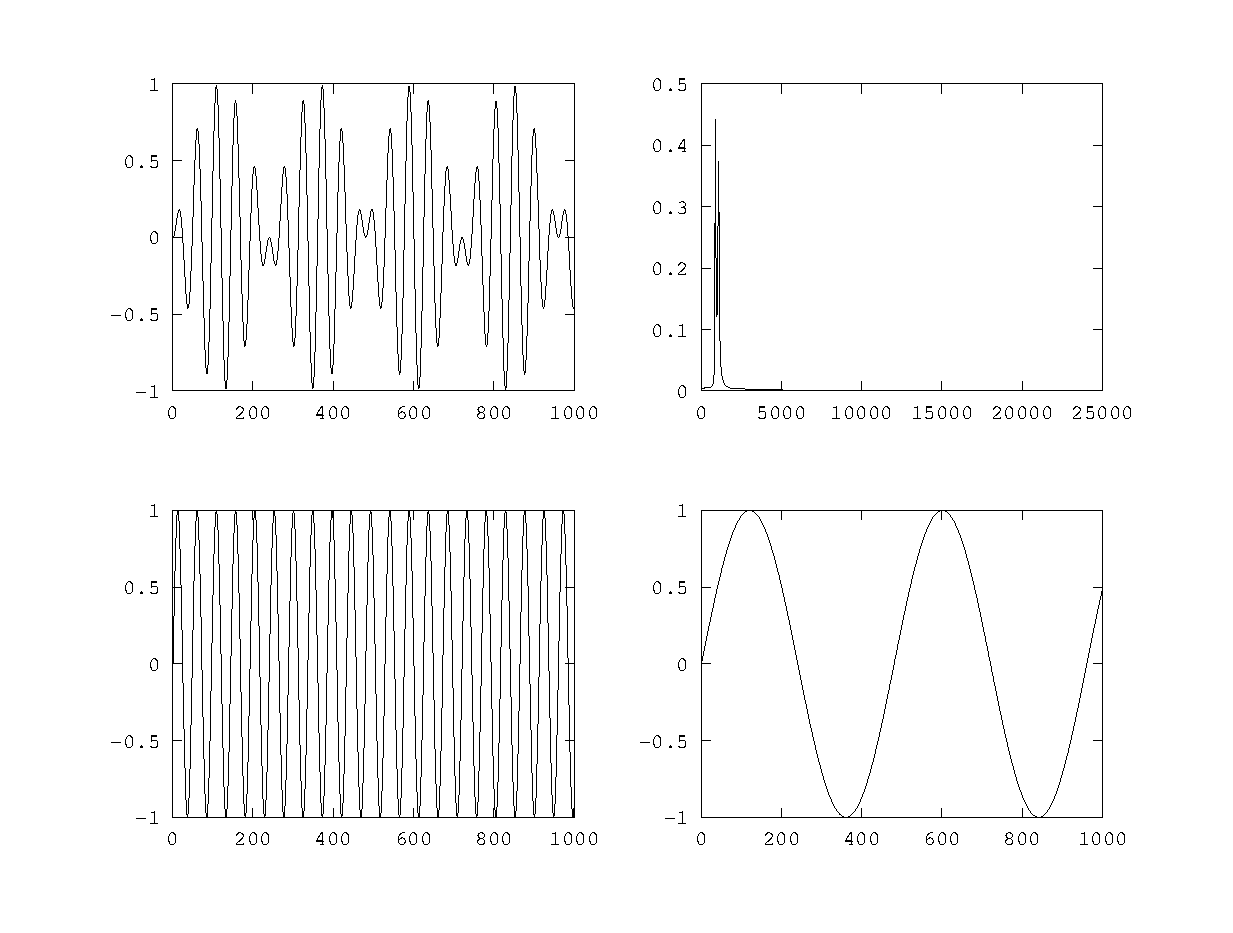
\includegraphics[scale=0.8]{proba3_dom}
\caption{Modulacja amplitudowa}
\label{fig:5}
\end{figure}
\end{enumerate}
\end{document}
